\section{Experiments and Results}
\label{sec:experiments}

\subsection{Datasets, models and protocol}
\label{sec:protocol}

\paragraph{Datasets.}
\Cref{tab:data} in \cref{app:data} lists the five datasets.
NYU Depth v2~\cite{silberman2012nyu} and KITTI~\cite{geiger2012kitti} are used throughout; on KITTI the ground truth is built from the same LiDAR that would provide anchors, so it cannot test an independent sensor.
DIODE~\cite{vasiljevic2019diode} and ETH3D~\cite{schops2017eth3d} test domain shift and the case of very few scenes.
ARKitScenes~\cite{baruch2021arkitscenes} (depth-upsampling validation split) provides an independent sensor.
Its ground truth is a Faro laser scan, while the deployed sensor is the iPad Pro LiDAR depth from ARKit (fused, with confidence classes $0,1,2$), which reads about \NumArkIpadOffset\% nearer than the laser.
Valid pixels are kept on a regular lattice (stride 4 on NYU, 2 on KITTI and DIODE, 8 on ARKitScenes) and stored per image, so per-image statistics are exact.
Every split is by scene: head-train (fits scores, $m$, $s$ and hyper-parameters), calibration (cross-scene thresholds; unused by \mDual) and test.
The main-method experiments use 30/35/35\%.


\paragraph{Frozen models.}
We use UniDepthV2-Large~\cite{piccinelli2025unidepthv2}, Depth Anything V2 Large metric~\cite{yang2024dav2} (indoor checkpoint on NYU, DIODE indoor and ARKitScenes; outdoor checkpoint on KITTI and DIODE outdoor), Depth Pro~\cite{bochkovskii2025depthpro} and Metric3D v2 ViT-Large~\cite{hu2024metric3dv2}.
Metric3D v2 is given the calibrated focal length, while the other three infer the camera, so it is not compared like for like.
NYU and KITTI are not in the training mixtures of these models.
UniDepthV2's training mixture includes ARKitScenes, which can affect width but not any guarantee; Depth Pro was trained on ARKitScenes and is not used there.
On ARKitScenes we also use the depth-completion network \omnidc~\cite{zuo2025omnidc} (v1.1, trained only on synthetic data).
It sees RGB and the structured anchors only, never the probes.
\Cref{fig:models} shows the ARKitScenes inputs and the two frozen models used there.

\begin{figure}[t]
\centering
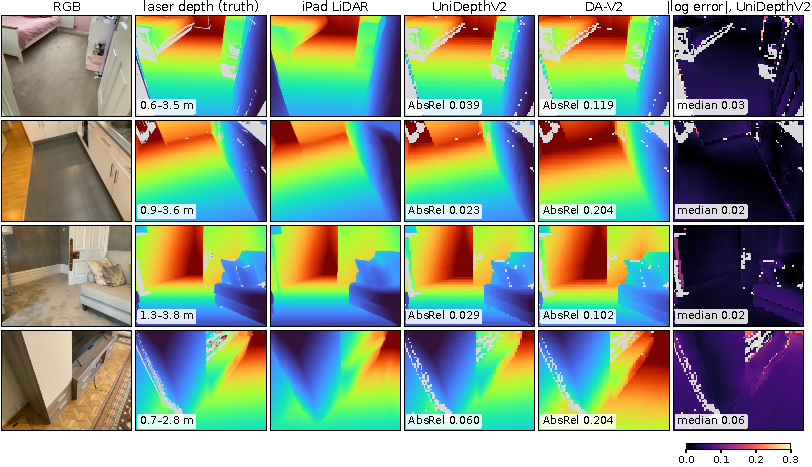
\includegraphics[width=\linewidth]{figures/models_qual.pdf}
\caption{\textbf{ARKitScenes: the reference, the deployed sensor and two frozen models} (four frames from different homes, chosen for their depth range, so their errors are below the dataset average of AbsRel \NumArkUniAbsRel{} for UniDepthV2 and \NumArkDavAbsRel{} for DA-V2). Depth panels of a row share one colour scale (range in the laser panel; grey: no value). The laser scan is the ground truth; the iPad LiDAR is smooth and reads slightly nearer. Predictions and the error map are shown on the evaluation lattice (stride 8). DA-V2 (indoor metric) overestimates depth throughout, the global scale error that anchors remove.}
\label{fig:models}
\end{figure}

\paragraph{Metrics.}
Coverage is image-averaged (\cref{eq:cov}).
Per-image spread is the 10th percentile (p10) of $\Cov_i$ and the share of \emph{short} images, whose coverage on one probe draw is below $1-\alpha-0.05=0.85$ (theory at $n=20$: \NumBetaShortOneTwenty\%).
Width is the median relative width; IS is the relative interval score of \cref{sec:problem}.
$\alpha=0.1$ unless stated.

\paragraph{Protocol and decision rules.}
The broad study used 20 random scene splits for the cross-image calibrators and 3--5 splits $\times$ 2--6 anchor draws for the anchor experiments.
A method was called \emph{valid} if its mean coverage over splits is at least $1-\alpha-2\,$SE.
It was called \emph{better} than another only if the 95\% paired bootstrap interval of their interval-score difference over splits excludes zero.
The dual-anchor experiments were first run in an exploratory phase (3 splits $\times$ 2 probe draws), which chose the shrinkage $\gamma=0.5$ after $\gamma=1$ showed a heavy width tail.
All comparisons are then replicated in a confirmatory run whose analysis plan was frozen before the runs: E17c (\NumReplSplits{} splits $\times$ \NumProbeDraws{} probe draws on NYU and KITTI, plus an $r=n$ arm), E18c (the same on ARKitScenes), E19c (10 visit splits, each with its own anchor mask) and E20 (the envelope).
The plan also fixes two thresholds in advance.
The completion centre ``wins'' a layout only if its best valid method beats UniDepthV2 $+$ \mDual by at least 15\% in IS.
The envelope enters the main method only if its truth coverage is valid and it beats \mDistBoth by at least 10\%.
Two amendments were logged before any affected output was seen: the primary IS definition, and the single-CRC envelope of \cref{sec:env}.

\subsection{Broad study: what conformal wrapping and anchors can and cannot do}
\label{sec:res:broad}

\Cref{tab:broad} summarizes the broad study; details and further tables are in \cref{app:broad}.

\begin{table}[t]
\centering\small
\caption{\textbf{Broad study (E0--E16), headline results.} Plain log score, $\alpha=0.1$; ranges over the NYU/KITTI $\times$ model pairs unless stated. The E13 row is re-measured by the confirmatory run (E17c).}
\label{tab:broad}
\footnotesize
\setlength{\tabcolsep}{3pt}
\begin{tabular}{@{}p{0.2\linewidth}p{0.77\linewidth}@{}}
\toprule
Experiment & Result \\
\midrule
E0 accuracy & AbsRel on NYU / KITTI: UniDepthV2 0.071 / 0.077, DA-V2 0.206 / 0.109, Depth Pro 0.092 / 0.139, Metric3D v2 0.066 / 0.048. \\
E2--E4 validity & Cross-image CRC (K1) covers 0.894--0.900 on every NYU/KITTI pair; raw uncertainties claiming 90\% cover 3--16\% (flip), 15--43\% (ensemble) and 83--91\% (learned variance). \\
E1, E8 units & Run-to-run SD of coverage follows the Beta law with $n=$ \#images and is ${\approx}100\times$ the pixel-count prediction (\cref{fig:units}). \\
Scene level & Image-event calibration is slightly short on scene-clustered data (0.884--0.897); its scene version meets the target (0.908--0.940) for 3--12\% more width. \\
E5 shift, ETH3D & Calibrating on one dataset and testing on another: 33--85\% coverage. On ETH3D (13 scenes) a scene-dependent scale bias drops Depth Pro to 0.69; scene-level calibration needs $\ge9$ calibration scenes and returns infinite intervals with 4. \\
E11 anchors & One global scale error explains \NumScaleVarLo--\NumScaleVarHi\% of image-to-image variation in coverage. About 20 random anchors match an oracle that knows each image's scale, giving intervals 1.1--3.7$\times$ narrower. \mLocal matches its exact theory (0.908--0.910 vs.\ 0.909 at $k=20$), and \mBoth cuts short images from 16\% to 0.2\% (NYU, DA-V2). \\
E13 structured & \mLocal on structured anchors covers \ESeventeen{cluster}{50}{local}/\ESeventeen{cluster}{200}{local} (cluster), \ESeventeen{near}{50}{local}/\ESeventeen{near}{200}{local} (near), \ESeventeen{rows}{50}{local}/\ESeventeen{rows}{200}{local} (rows; $k=50/200$, median over pairs, E17c), with \emph{narrower} intervals. Cross-image \mRescale and \mHybrid stay valid under every layout. \\
E14 \mDist & Coverage is flat across distance to the nearest anchor under all five layouts, and up to 67\% narrower than \mHybrid. With 20 of the $k$ anchors spent at random, \mDistBoth covers 0.965--0.983 with $\le$0.3\% short images. \\
E15 mismatch & Calibrating under one layout and deploying another leaves coverage as low as 0.77 (\mHybrid, edges $\to$ cluster). The largest threshold over layouts (@max) is valid for each layout. LSCP covers 0.17--0.93, depending on the layout. \\
E16 noise & With matched sensor noise, every cross-image guarantee holds (0.916--0.925). Calibrating on clean anchors fails under outliers (\mDist 0.66) and a 5\% bias (0.36--0.86). Within-image methods cover the sensor reading, so a bias breaks them (0.38--0.78). \\
E12 safety & Only guarantees calibrated on the query itself (nearest depth in a region) are valid and informative. Per-pixel guarantees leave the region minimum over-estimated in 2--24\% of images, and simultaneous coverage of all pixels raises alarms on 99--100\% of safe images. \\
\bottomrule
\end{tabular}
\end{table}

\begin{figure}[t]
\centering
\begin{minipage}[t]{0.47\linewidth}
\centering
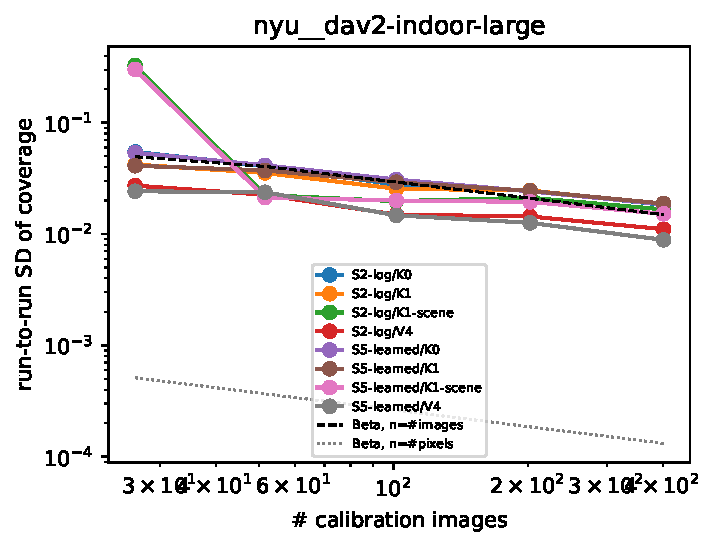
\includegraphics[width=\linewidth]{e8_calsize__nyu__dav2-indoor-large.pdf}
\captionof{figure}{\textbf{The image is the unit (E8, NYU, DA-V2).} Run-to-run SD of coverage against the number of calibration images (50 splits). Dashed: Beta law with $n=$ \#images; dotted: with $n=$ \#pixels.}
\label{fig:units}
\end{minipage}\hfill
\begin{minipage}[t]{0.49\linewidth}
\footnotesize
\textbf{Reading the findings.}
Conformal wrapping fixes \emph{average} coverage everywhere at modest cost, and the score matters: learned or relative scores give up to 20\% lower interval score.
What cross-image calibration cannot fix is the spread of coverage across individual images (16\% of NYU images short with DA-V2), or a change of dataset without target calibration data.
Anchors attack the dominant per-image error, the global scale.
Within-image calibration then gives a per-image guarantee that needs no calibration set at all (on DIODE it is the only finite option: 0.900 coverage at $k=200$).
But it holds only for random anchors, and every failure under structured anchors is \emph{silent}: the intervals look tighter, not looser.
\end{minipage}
\end{figure}

\paragraph{Pixels are not the unit (Q1).}
On synthetic data with a controllable per-image scale error, average coverage stays at 0.90 while the spread of per-image coverage grows from 0.006 to 0.195: average validity says nothing about individual images.
On real data the run-to-run variability tracks the image-count prediction within a factor of 0.8--1.7 (\cref{fig:units}).
With few, very different scenes (ETH3D, 4 calibration scenes per split) the small slip of image-level guarantees becomes a collapse, and the valid scene-level version is uninformative.

\paragraph{Structured anchors break within-image calibration (Q2).}
Cross-image anchor methods stay valid under every layout, because calibration and test share it, at a width cost (clustered anchors make \mHybrid 26--61\% wider than random anchors at $k=20$).
\mLocal fails, and with it \mBoth's per-image guarantee: under clustered or near-only anchors 5--14\% of \mBoth's images fall below 0.80, against 0.3--2\% with random anchors.
Coverage also falls with distance to the nearest anchor even for random anchors, from \NumLocalNearBinCovLo--\NumLocalNearBinCovHi{} next to an anchor to \NumLocalFarBinCovLo--\NumLocalFarBinCovHi{} at 0.1--0.2 of the image diagonal.

\begin{figure}[t]
\centering
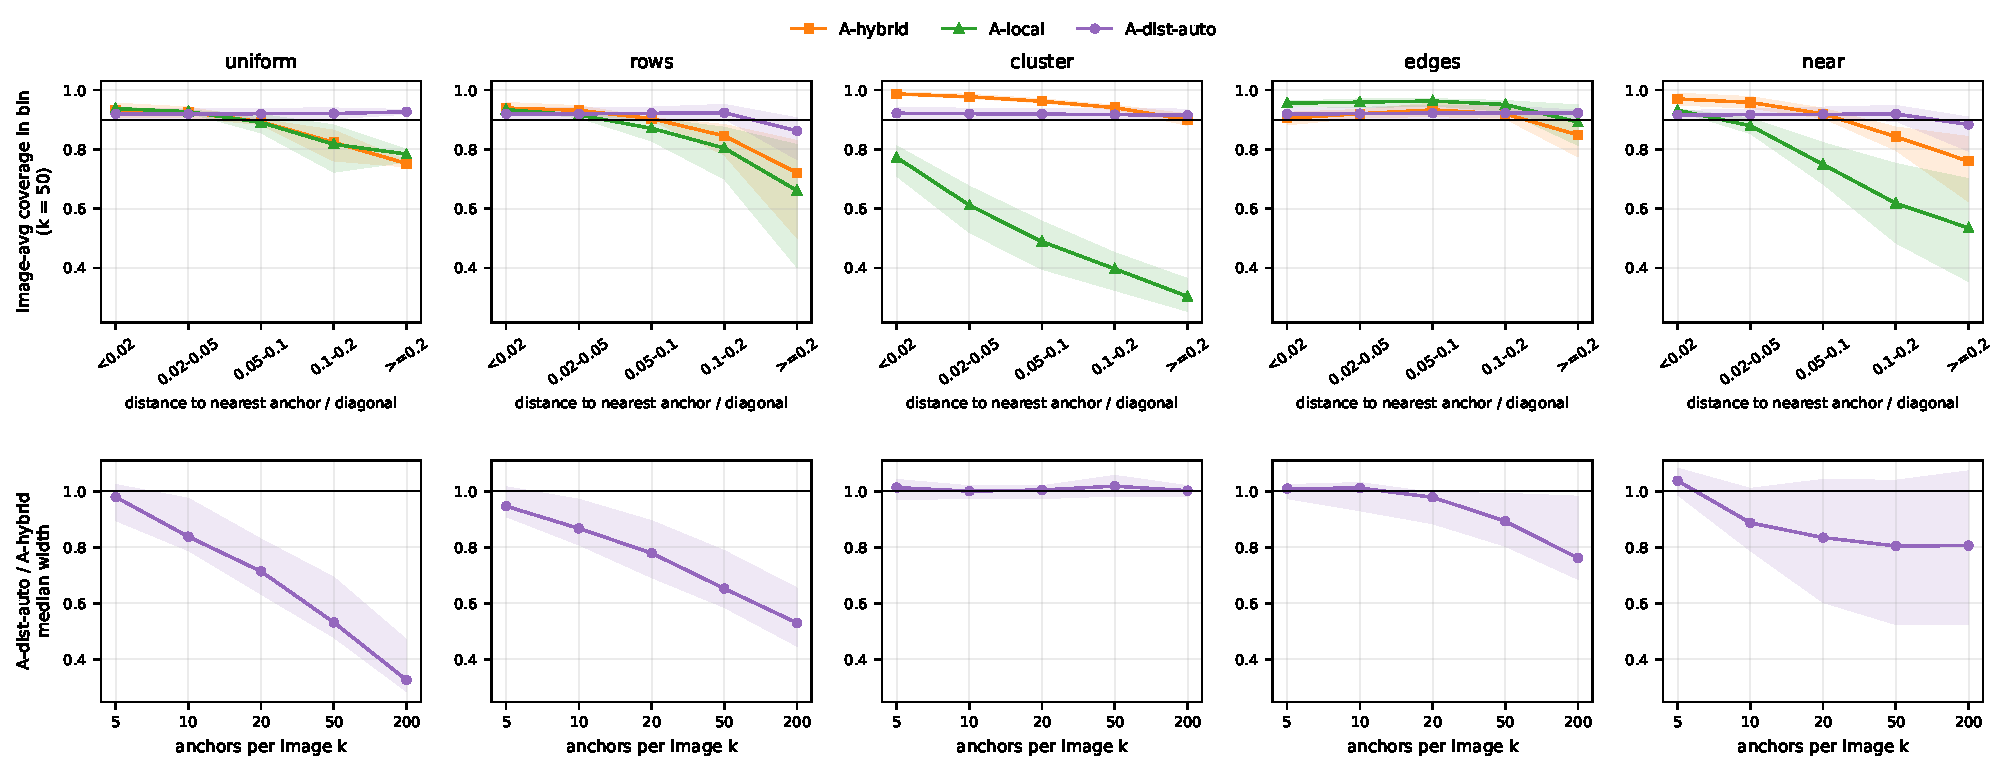
\includegraphics[width=0.9\linewidth]{e14_distance__S2-log.pdf}
\caption{\textbf{Distance-aware anchors (E14).} Top: image-averaged coverage per bin of distance to the nearest anchor ($k=50$; mean over the six NYU/KITTI pairs, band: min--max; line: 0.9). \mLocal collapses with distance under structured layouts; \mDist stays flat under all five. Bottom: \mDist's median width relative to \mHybrid against the number of anchors.}
\label{fig:adist}
\end{figure}

\paragraph{The distance-aware model and its limits.}
\mDist removes the distance gradient (\cref{fig:adist}).
At $k=20$ under uniform anchors its farthest-bin coverage is 0.86--0.91, where \mHybrid's is 0.66--0.83.
It is narrower wherever the anchors spread over the image (uniform: $-29\%$ at $k=20$, $-67\%$ at $k=200$; rows: up to $-47\%$) and within 6\% of \mHybrid under clusters.
Its guarantee is still an average over scenes, and it inherits two weaknesses of cross-image calibration.
Under a layout mismatch it misses by up to 4 points on average (0.863, near $\to$ edges); @max calibration fixes this at a width cost.
With noisy anchors, calibrating on clean data is unsafe: with 10\% outliers it covers 0.66 at $k=200$, and next to the anchors only 0.63.
Spending 20 measurements at random and taking the hull with \mLocalSplit (\mDistBoth) restores a per-image guarantee under every layout.
This budget split is the seed of the main method: the random measurements do the calibrating, so the structured ones need not.

\subsection{Main method: structured anchors break reused calibration; probes restore it}
\label{sec:res:failure}
\label{sec:res:dual}

\begin{table}[t]
\centering\footnotesize
\caption{\textbf{NYU and KITTI, three frozen models (UniDepthV2, DA-V2, Depth Pro), $n=20$ probes, $\alpha=0.1$} (confirmatory E17c, \NumReplSplits{} scene splits $\times$ \NumProbeDraws{} probe draws); median over the six model--dataset pairs. \textsf{local}: \mLocal calibrated on the $k$ structured anchors themselves; \textsf{dual}: \mDual; \textsf{both}: \mDualBoth. Short: \% of images whose coverage on one probe draw is below 0.85. $\Delta$: change in median relative width and relative IS (primary) against \mDistBoth. $^\dagger$Uniform anchors only. $^\ddagger$\Cref{tab:budget}.}
\label{tab:main}
\setlength{\tabcolsep}{4pt}
\newcommand{\rowE}[3]{#1 & #3 & \ESeventeen{#2}{#3}{local} & \ESeventeen{#2}{#3}{dual} & \ESeventeen{#2}{#3}{short} & \ESeventeen{#2}{#3}{dW} & \ESeventeen{#2}{#3}{bW} & \ESeventeen{#2}{#3}{dIS} & \ESeventeen{#2}{#3}{bIS} \\}
\begin{tabular}{@{}llccccccc@{}}
\toprule
 & & \multicolumn{2}{c}{Coverage} & Short (\%) & \multicolumn{2}{c}{$\Delta$ width (\%)} & \multicolumn{2}{c}{$\Delta$ IS (\%)} \\
\cmidrule(lr){3-4}\cmidrule(lr){5-5}\cmidrule(lr){6-7}\cmidrule(l){8-9}
Layout & $k$ & \textsf{local} & \textsf{dual} & \textsf{dual} & \textsf{dual} & \textsf{both} & \textsf{dual} & \textsf{both} \\
\midrule
\rowE{uniform}{uniform}{50}\rowE{}{uniform}{200}
\midrule
\rowE{rows}{rows}{50}\rowE{}{rows}{200}
\midrule
\rowE{cluster}{cluster}{50}\rowE{}{cluster}{200}
\midrule
\rowE{edges}{edges}{50}\rowE{}{edges}{200}
\midrule
\rowE{near}{near}{50}\rowE{}{near}{200}
\midrule
\multicolumn{2}{@{}l}{theory} & $\ge$0.9$^\dagger$ & \NumDualCovTheory & \NumBetaShortOneTwenty$^\ddagger$ & & & & \\
\bottomrule
\end{tabular}
\end{table}

\paragraph{Failure (\cref{tab:main}, \textsf{local}).}
Calibrating within the image on the structured anchors themselves keeps nominal coverage only for uniform anchors.
Under clustered anchors it covers \ESeventeen{cluster}{50}{local} and \ESeventeen{cluster}{200}{local} at $k=50$ and 200 (medians over the six pairs; range over pairs and both budgets \NumLocalClusterCovLo--\NumLocalClusterCovHi); under near-only anchors \ESeventeen{near}{50}{local} and \ESeventeen{near}{200}{local}; under scan lines \ESeventeen{rows}{200}{local} at $k=200$.
Edge anchors over-cover, since edges are where errors are largest.
The failing intervals are narrower, not wider: with 50 clustered anchors their median relative width is \NumLocalClusterWidthLo--\NumLocalClusterWidthHi, against \NumLocalUnifWidthLo--\NumLocalUnifWidthHi{} for uniform ones.
Even uniform anchors hide a spatial gap: at $k=50$, coverage falls from \NumLocalNearBinCovLo--\NumLocalNearBinCovHi{} within 0.02 of the image diagonal from an anchor to \NumLocalFarBinCovLo--\NumLocalFarBinCovHi{} at 0.1--0.2 of it.
\Cref{fig:layouts} shows both effects on one frame.

\begin{figure}[t]
\centering
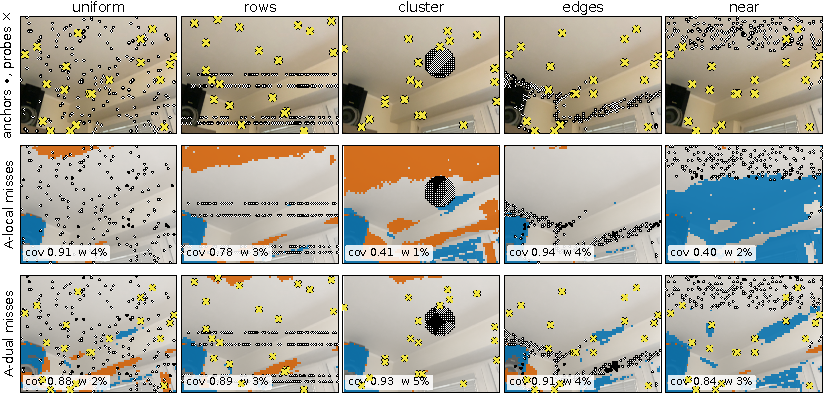
\includegraphics[width=\linewidth]{figures/layouts_qual.pdf}
\caption{\textbf{One ARKitScenes test frame under the five anchor layouts} (UniDepthV2, $k=200$: 180 structured anchors $\bullet$ and 20 probes $\times$, laser values, split 0, one draw). Rows 2--3: pixels whose true depth lies outside the interval (vermillion: truth farther, blue: nearer); cov: coverage of the frame's evaluation pixels; w: median relative width. \mLocal, calibrated on the structured anchors, holds only where they are representative: under clustered and near-only anchors it covers 0.41 and 0.40 with intervals 1--2\% wide. \mDual, calibrated on the probes, stays near 0.9 in every layout; its frame-to-frame spread around $0.905$ is the law of \cref{prop:budget}.}
\label{fig:layouts}
\end{figure}

\paragraph{Separating the roles restores per-image validity.}
\mDual covers \NumDualCovLo--\NumDualCovHi{} in every layout, $k$ and pair, at its theoretical rate $r/(n+1)=\NumDualCovTheory$ (within two standard errors in \NumDualExactCells{} of the \NumAllCells{} pair--layout--$k$ cells).
It is at least 10\% narrower than the hull baseline \mDistBoth on \NumDualGatePairs{} of \NumPairs{} pairs in each of the \NumCells{} layout--$k$ cells, and \NumDualWidthGainLo--\NumDualWidthGainHi\% narrower overall (median over pairs; paired bootstrap intervals exclude 0).
Part of that width is \mDistBoth's over-coverage (\NumDistBothCovLo--\NumDistBothCovHi), so the interval score, which charges misses, is the fairer comparison.
On it \mDual is better in \NumDualISWins{} of the \NumAllCells{} cells, including every cell with uniform or scan-line anchors (by \NumDualISGainURLo--\NumDualISGainURHi\%); \mDistBoth is better in \NumDualISLosses, nine of them clustered, by at most \NumDualISLoseMax\%.
\mDualBoth is better than \mDistBoth in \NumDualBothISWins{} cells and worse in \NumDualBothISLosses, all clustered and by at most \NumDualBothISLoseMax\%.
Under clustered anchors its two halves are centred differently and it gains only \NumDualBothClusterWidthLo--\NumDualBothClusterWidthHi\% in width.
\mDual's coverage varies across distance bins by \NumSpreadDualLo--\NumSpreadDualHi{} points; \mDualBoth reduces this to \NumSpreadDualBothLo--\NumSpreadDualBothHi{} (\cref{fig:dual}a).

\begin{figure}[t]
\centering
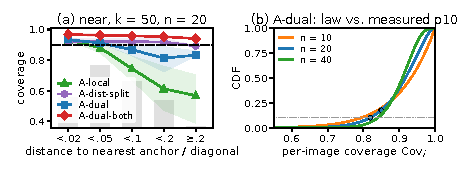
\includegraphics[width=0.8\linewidth]{figures/e17_results.pdf}
\caption{\textbf{What each guarantee protects (E17).} (a)~Near layout, $k=50$, $n=20$: \mDual's coverage decreases with distance, as \cref{thm:dual} allows; \mDualBoth is flat. Lines/bands: median/range over the six NYU/KITTI pairs; bars: pixel share; dashed: 0.9. (b)~CDF of the per-image coverage law (\cref{prop:budget}) for $n=10,20,40$ (theory); dots, $n=20$: measured p10 of $\Cov_i$ at 0.1 and measured share of short images at 0.85 (median over pairs, layouts and $k$; bars: range).}
\label{fig:dual}
\end{figure}

\paragraph{The probe budget.}
With 20 probes the 10th percentile of $\Cov_i$ was \NumMeasPTenTwenty{} (law: \NumBetaPTenTwenty), an implementation check of the randomization (\cref{fig:dual}b).
With 10 probes \mDistBoth is infinite on every image by construction; 40 probes tighten the law only slowly at twice the measurement cost, so we keep $n=20$ (\cref{app:budget}).

\subsection{Which centre to calibrate: a depth-completion network or the frozen model (E19c)}
\label{sec:res:omni}

\begin{table}[t]
\centering\footnotesize
\caption{\textbf{ARKitScenes, which centre to calibrate (E19c, confirmatory).} $k=200$ (180 structured anchors $+$ 20 probes), laser-valued anchors and probes, $\alpha=0.1$; mean over ten visit splits, one probe draw each. UniDepthV2 is frozen; \omnidc is completed from RGB and the 180 anchors. \mSplitCP calibrates one quantile on dense laser depth of calibration scenes; the UniDepthV2 \mSplitCP row uses no anchors. W$/y$: median width over laser depth; IS: primary relative interval score. Theory for \mDual, one draw: coverage \NumDualCovTheory, p10 \NumBetaPTenTwenty.}
\label{tab:omni}
\setlength{\tabcolsep}{3.5pt}
\newcommand{\eO}[3]{\ENineteen{#1}{#2}{clean}{clean}{#3}{cov} & \ENineteen{#1}{#2}{clean}{clean}{#3}{ptten} & \ENineteen{#1}{#2}{clean}{clean}{#3}{wgt} & \ENineteen{#1}{#2}{clean}{clean}{#3}{is}}
\newcommand{\rowO}[3]{#1 & #3 & \eO{uniform}{#2}{#3} & \eO{cluster}{#2}{#3} \\}
\begin{tabular}{@{}llcccc@{\hspace{8pt}}cccc@{}}
\toprule
 & & \multicolumn{4}{c}{Uniform layout} & \multicolumn{4}{c}{Cluster layout} \\
\cmidrule(lr){3-6}\cmidrule(l){7-10}
Centre & Calibration & Cov. & p10 & W$/y$ & IS & Cov. & p10 & W$/y$ & IS \\
\midrule
\rowO{UniDepthV2}{unidepth}{split-CP}
\midrule
\rowO{UniDepthV2 + $\cS$}{unidepth}{A-dist-split}
\rowO{}{unidepth}{A-dual}
\rowO{}{unidepth}{A-dual-both}
\midrule
\rowO{\omnidc + $\cS$}{omnidc}{split-CP}
\rowO{}{omnidc}{A-dist-split}
\rowO{}{omnidc}{A-dual}
\rowO{}{omnidc}{A-dual-both}
\bottomrule
\end{tabular}
\end{table}

\paragraph{Uniform anchors: the completion network is the better centre.}
\mSplitCP, \mDual and \mDistSplit on \omnidc's output have a \NumOmniGainLo--\NumOmniGainHi\% lower IS than \mDual on UniDepthV2 (\cref{tab:omni}; all paired intervals exclude zero).
This fires the pre-specified $\ge$15\% criterion, so the layer belongs on top of the completion network.
\mDual on \omnidc costs \NumOmniDualCost\% in IS over \mSplitCP on the same output and adds the per-image law: p10 \ENineteen{uniform}{omnidc}{clean}{clean}{A-dual}{ptten} and \ENineteen{uniform}{omnidc}{clean}{clean}{A-dual}{short}\% short images, as \cref{tab:budget} predicts.
\mSplitCP has no per-image guarantee and needs dense reference depth on calibration scenes.
Without anchors, \mSplitCP on the frozen model has \NumRawRatioLo--\NumRawRatioHi$\times$ the IS of any anchored method under uniform anchors, and 1.3--3.9$\times$ under clustered anchors.

\paragraph{Clustered anchors: the ranking reverses.}
Away from the one observed patch, the completion network extrapolates poorly.
\mSplitCP on its output is not valid (coverage \ENineteen{cluster}{omnidc}{clean}{clean}{split-CP}{cov}, more than 2\,SE below 0.9, p10 \ENineteen{cluster}{omnidc}{clean}{clean}{split-CP}{ptten}).
\mDual on UniDepthV2 has a \NumClusterGainDual\% lower IS than \mDual on \omnidc, and a \NumClusterGainCP\% lower IS than \mSplitCP on \omnidc.
On \omnidc itself, \mDual beats \mSplitCP by 17\%.
On the frozen centre, \mDistSplit is more efficient still (IS \ENineteen{cluster}{unidepth}{clean}{clean}{A-dist-split}{is}) but has no per-image guarantee, while \mDualBoth keeps both guarantees at \ENineteen{cluster}{unidepth}{clean}{clean}{A-dual-both}{is}.
Across both centres and layouts, \mDual's per-image spread is the same (p10 \NumENineteenPTenLo--\NumENineteenPTenHi, \NumENineteenShortLo--\NumENineteenShortHi\% short), as \cref{thm:dual} requires of any probe-independent centre.

\paragraph{Point accuracy agrees.}
On the test pixels outside the structured anchors (image-mean AbsRel, mean over the ten splits), \omnidc reaches 0.0064 under uniform and 0.0738 under clustered anchors.
UniDepthV2 rescaled per image by the median $\log(y/\yhat)$ at the same 180 anchors reaches 0.0293 and 0.0394, and 0.121 without anchors.
$\delta<1.25$ is 0.997 vs.\ 0.988 (uniform) and 0.944 vs.\ 0.981 (cluster).
So under uniform anchors \omnidc is about $4.6\times$ more accurate, while under clustered anchors a single per-image scale on the frozen model halves \omnidc's error.
This supports the interval-score result independently.
A mean-over-images IS would instead be dominated by a few \omnidc pixels with extreme upper bounds under clustered anchors (\cref{app:blowup}).

\subsection{What the probes certify: an independent sensor (E18)}
\label{sec:res:sensor}

\begin{table}[t]
\centering\footnotesize
\caption{\textbf{Laser-truth coverage by value source of anchors / probes} (ARKitScenes, $k=200$, $\alpha=0.1$; L $=$ laser, I $=$ iPad LiDAR). Frozen-model rows: confirmatory E18c, mean over \NumReplSplits{} visit splits and ten probe draws; \mDualEnv: E20, same splits and draws, iPad probes only. \omnidc rows: E19c, ten splits; \omnidc completed from iPad anchors (I/L, I/I) was not part of the confirmatory run (--).}
\label{tab:sensor}
\setlength{\tabcolsep}{4pt}
\newcommand{\eB}[3]{\ENineteen{#1}{#2}{clean}{clean}{#3}{cov} & -- & \ENineteen{#1}{#2}{clean}{lidar}{#3}{cov} & --}
\newcommand{\rowB}[3]{#1 & #3 & \eB{uniform}{#2}{#3} & \eB{cluster}{#2}{#3} \\}
\newcommand{\eC}[3]{\EEighteen{#1}{#2}{clean}{clean}{#3}{cov} & \EEighteen{#1}{#2}{lidar}{clean}{#3}{cov} & \EEighteen{#1}{#2}{clean}{lidar}{#3}{cov} & \EEighteen{#1}{#2}{lidar}{lidar}{#3}{cov}}
\newcommand{\rowC}[3]{#1 & #3 & \eC{uniform}{#2}{#3} & \eC{cluster}{#2}{#3} \\}
\newcommand{\eEnv}[2]{-- & -- & \ETwenty{#1}{#2}{clean}{A-dual-env}{cov} & \ETwenty{#1}{#2}{lidar}{A-dual-env}{cov}}
\newcommand{\rowEnv}[1]{ & \mDualEnv & \eEnv{uniform}{#1} & \eEnv{cluster}{#1} \\}
\begin{tabular}{@{}llcccc@{\hspace{10pt}}cccc@{}}
\toprule
 & & \multicolumn{4}{c}{Uniform layout} & \multicolumn{4}{c}{Cluster layout} \\
\cmidrule(lr){3-6}\cmidrule(l){7-10}
Centre & Calibration & L/L & I/L & L/I & I/I & L/L & I/L & L/I & I/I \\
\midrule
\rowC{UniDepthV2 + $\cS$}{unidepth}{A-dist-split}
\rowC{}{unidepth}{A-local-split}
\rowC{}{unidepth}{A-dual}
\rowC{}{unidepth}{A-dual-both}
\rowC{}{unidepth}{A-dist-both}
\rowEnv{unidepth}
\midrule
\rowC{DA-V2 + $\cS$}{dav2}{A-dist-split}
\rowC{}{dav2}{A-local-split}
\rowC{}{dav2}{A-dual}
\rowC{}{dav2}{A-dual-both}
\rowC{}{dav2}{A-dist-both}
\rowEnv{dav2}
\midrule
\rowB{\omnidc + $\cS$}{omnidc}{split-CP}
\rowB{}{omnidc}{A-dist-split}
\rowB{}{omnidc}{A-dual}
\bottomrule
\end{tabular}
\end{table}

\Cref{tab:sensor} varies what the measurements report, with coverage always measured against the laser.
With laser probes, \mDual's spread on ARKitScenes, over UniDepthV2 and DA-V2 (AbsRel \NumArkUniAbsRel{} and \NumArkDavAbsRel) and both layouts, is as predicted (p10 \NumEEighteenPTen, short \NumEEighteenShort).
This is a check on data that were not used to choose $\gamma$.
\begin{itemize}[leftmargin=*,itemsep=1pt,topsep=2pt]
\item \emph{iPad anchors, laser probes:} \mDual covers the laser truth at \NumEEighteenCovIL{} in both layouts, with the clean-value spread (p10 \NumEEighteenPTen), because the probes measure the truth and absorb the anchors' bias into the threshold.
\mDistSplit, calibrated on the values the measurements report, covers it at only \NumEEighteenDistIpad{} under uniform anchors with iPad anchors (either probe source).
\item \emph{Laser anchors, iPad probes:} \mDual over-covers (\NumEEighteenCovLI{} uniform), with \NumEEighteenWiden$\times$ wider intervals, as the iPad's own errors enter the threshold.
\item \emph{iPad values for both}, the deployed configuration without a reference: \mDual certifies the iPad reading.
Under uniform anchors its intervals are about as narrow as the \NumArkIpadOffset\% sensor bias, and it covers the laser truth at only \NumEEighteenCovII{} (p10 \NumEEighteenPTenII).
The wider cluster intervals absorb more (\NumEEighteenCovIICluster), and the hull \mDualBoth recovers the truth there (\NumEEighteenHullIICluster) but not under uniform anchors (\NumEEighteenHullII).
Calibration within the image behaves the same: \mLocalSplit covers the truth at \NumEEighteenLocalSplitLaserLo{} with laser probes and \NumEEighteenLocalSplitIpadLo--\NumEEighteenLocalSplitIpadHi{} with iPad probes, in both layouts.
\end{itemize}
\Cref{fig:sensor} shows why on three frames: the iPad reads a few per cent nearer than the laser over much of a frame, so probes that report the iPad calibrate intervals around the iPad's depth, and the laser truth falls beyond them.

\begin{figure}[t]
\centering
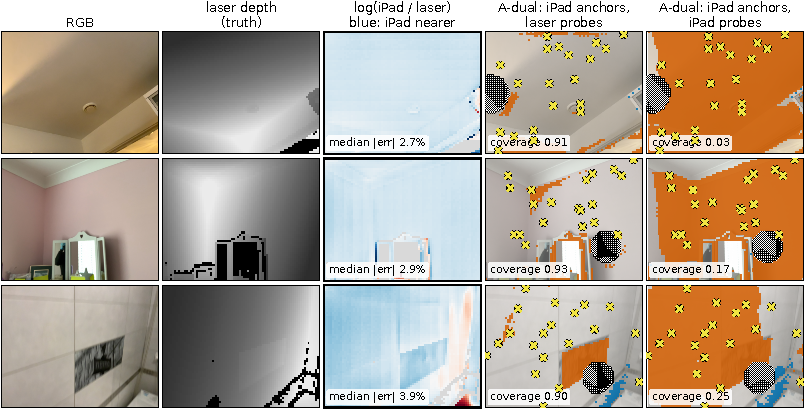
\includegraphics[width=\linewidth]{figures/sensor_qual.pdf}
\caption{\textbf{Probe source and truth coverage} (three ARKitScenes test frames from different visits; UniDepthV2, clustered layout, 180 structured anchors ($\bullet$, one cluster) reporting the iPad value, 20 probes ($\times$); split 0, one draw). Third column: log ratio of the iPad LiDAR to the laser depth (blue: iPad nearer; grey: no value). Right two columns: \mDual's misses of the laser truth (vermillion: truth farther than the interval, blue: nearer; dark grey: no ground truth), with laser and with iPad probes. Frames chosen among those whose coverage drops most from laser to iPad probes while staying near 0.9 with laser probes; averages over all frames are in \cref{tab:sensor}.}
\label{fig:sensor}
\end{figure}
Only \mDistBoth covers the truth in every cell of \cref{tab:sensor} (\EEighteen{uniform}{unidepth}{lidar}{lidar}{A-dist-both}{cov}--\EEighteen{uniform}{dav2}{clean}{clean}{A-dist-both}{cov}), and it does so through width, at \NumEEighteenDistBothRatio$\times$ \mDual's IS under uniform anchors with laser values (IS not shown).
\mSplitCP on \omnidc stays near nominal because it calibrates on laser depth of other scenes, which a deployed system lacks, but it is not valid under clustered anchors (\cref{sec:res:omni}).
Probes certify what they measure.

\paragraph{The sensor-error envelope (E20).}
The envelope of \cref{sec:env} restores truth coverage with iPad probes (\NumEnvTruthCov{} over both models, layouts and anchor sources), but it over-covers: its IS is \NumEnvISWorse{} above that of \mDistBoth (uniform \NumEnvISWorseUni, clustered \NumEnvISWorseCluster).
It therefore fails the gate fixed in advance (valid truth coverage and an IS at least 10\% below \mDistBoth) in both layouts, and \mDistBoth remains the cheaper way to cover the truth with sensor-grade probes.
The union bound behind \cref{prop:env} is loose here: \mDual at level $0.95$ already covers most of the truth, and widening every interval by the class band adds the rest again.
